
\section{Phasors}
	
    \begin{frame}{Phasors}
        \begin{itemize}
            \item Phasors express the response of a circuit to a sinusoidal input
            \item Any real, periodic signal can be expresses as the sum of sinusoids - we can apply this technique very broadly!
            \item A phasor encodes information about amplitude and phase, but not frequency
            $$v_s=A\cos(\omega t+\phi) \rightarrow \tilde{V}_s=Ae^{j\phi}$$
        \end{itemize}
    \end{frame}
    
    \begin{frame}{Impedance}
        \begin{itemize}
            \item Impedance ($Z$) is a generalized form of resistance - expresses a component's response to an alternating current
            \item Each common passive circuit element (resistor, capacitor, and inductor) has a characteristic impedance
            $$Z_R=R$$
            $$Z_C=\frac{1}{j\omega C}$$
            $$Z_L=j\omega L$$
        \end{itemize}
    \end{frame}
    
    \begin{frame}{Phasor Analysis Procedure}
        \begin{enumerate}
            \item Express all time domain signals as cosines
            \item Convert voltages, currents, and impedances to their phasor equivalents
            \item Set up phasor equations and solve for unknowns
            \item Transform back to time domain
        \end{enumerate}
    \end{frame}
    
    \begin{frame}{Phasor Practice}
        \begin{center}
            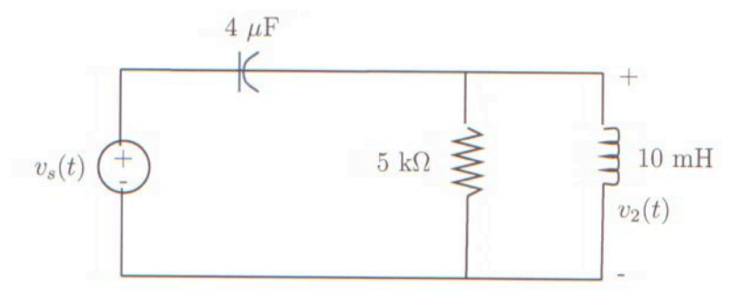
\includegraphics[width=0.5\textwidth]{./images/phasor-practice.png}
        \end{center}
        Let $v_s(t)=5\cos(5000t+\frac{\pi}{4})$. Find $v_2(t)$.
    \end{frame}

    \begin{frame}{Phasor Practice}
        \begin{center}
            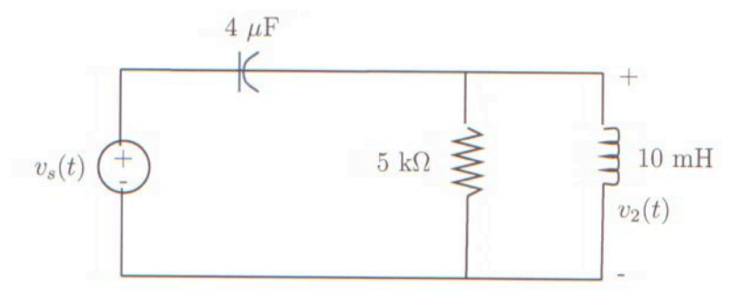
\includegraphics[width=0.5\textwidth]{./images/phasor-practice.png}
        \end{center}
        \begin{enumerate}
            \item Translate to phasor domain
            \begin{itemize}
                \item $\omega=5000$
                \item $v_s(t)=5\cos(5000t+\frac{\pi}{4})\rightarrow \tilde{V}_s=5e^{j\frac{\pi}{4}}$
                \item $C=4\mu F\rightarrow Z_C=\frac{1}{j(4*10^{-6})(5000)}=-j50$
                \item $R=5k\Omega\rightarrow Z_R=5*10^3$
                \item $L=10mH\rightarrow Z_L=j(5000)(10*10^{-3})=j50$
            \end{itemize}
        \end{enumerate}
    \end{frame}
    
    \begin{frame}{Phasor Practice}
        \begin{center}
            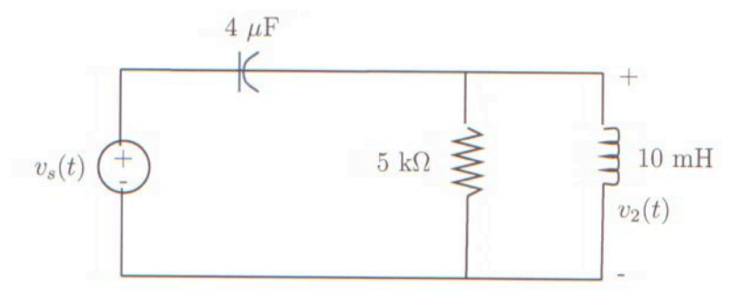
\includegraphics[width=0.5\textwidth]{./images/phasor-practice.png}
        \end{center}
        \begin{enumerate}
            \item[2.] Solve for $\tilde{V}_2$
            \begin{itemize}
                \item Set up as impedance divider: $$\frac{\tilde{V}_s}{Z_C+(Z_R\| Z_L)}=\frac{\tilde{V}_2}{Z_R\| Z_L}$$
                $$\tilde{V}_2=\tilde{V}_s\frac{Z_R\|Z_L}{Z_C+(Z_R\|Z_L)}=\tilde{V}_s\frac{\frac{Z_RZ_L}{Z_R+Z_L}}{\frac{Z_RZ_L+Z_RZ_C+Z_LZ_C}{Z_R+Z_L}}$$
            \end{itemize}
        \end{enumerate}
    \end{frame}
    
    \begin{frame}{Phasor Practice}
        \begin{center}
            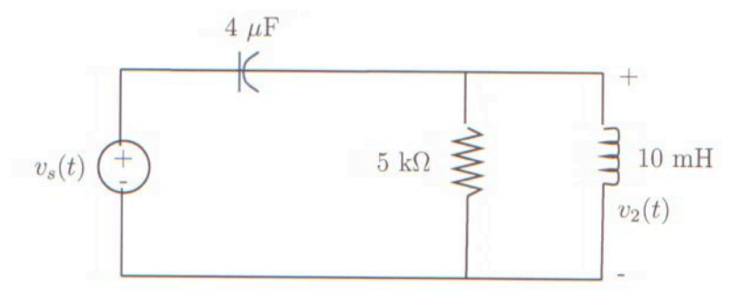
\includegraphics[width=0.5\textwidth]{./images/phasor-practice.png}
        \end{center}
        \begin{enumerate}
            \item[2.] Solve for $\tilde{V}_2$
            $$\tilde{V}_2=\tilde{V}_s\frac{Z_RZ_L}{Z_RZ_L+Z_RZ_C+Z_LZ_C}=\tilde{V}_s\frac{j2.5*10^5}{j2.5*10^5-j2.5*10^5+2500}$$
            $$\tilde{V}_2=j100\tilde{V}_s=100\tilde{V}_se^{j\frac{\pi}{2}}$$
        \end{enumerate}
    \end{frame}
    
    \begin{frame}{Phasor Practice}
        \begin{center}
            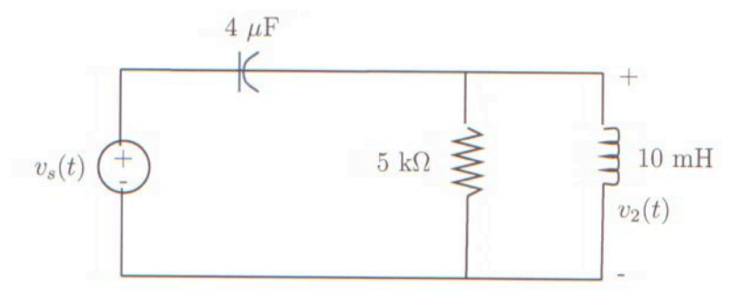
\includegraphics[width=0.5\textwidth]{./images/phasor-practice.png}
        \end{center}
        \begin{enumerate}
            \item[3.] Find time-domain solution
            \begin{itemize}
                \item $\tilde{V}_2=100e^{j\frac{\pi}{2}}\tilde{V}_s\rightarrow v_2(t)=100v_s(t+\frac{\pi}{2})=500\cos(5000t+\frac{3\pi}{4})$
            \end{itemize}
        \end{enumerate}
    \end{frame}
	
